\documentclass{standalone}
\usepackage{ tikz }
\usepackage{ xparse }
\input{macros/all}
\usepackage{amssymb}


\begin{document}
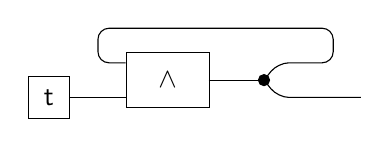
\begin{tikzpicture}[yscale=-1,x=1em,y=1.25em]
        

    \node [draw, minimum width=1.5em, minimum height=1.5em, anchor=east] at (-1,1) {$\mathsf{t}$};
    \draw (-1,1) -- (1,1);
    \node [draw, minimum width=3em, minimum height=2em, anchor=west] at (1,0.5) {$\land$};
    \draw (4,0.5) -- (6,0.5);
    \filldraw (6,0.5) circle (2pt);
    \draw [rounded corners] (6,0.5) -- (6.5,0) -- (8.5,0) -- (8.5,-1) -- (0,-1) -- (0,0) -- (1,0);
    \draw [rounded corners] (6,0.5) -- (6.5,1) -- (9.5,1);

\end{tikzpicture}
\end{document}